\documentclass[12pt,letterpaper]{hmcpset}
\usepackage[margin=1in]{geometry}
\usepackage{graphicx}
\usepackage[makeroom]{cancel}
\usepackage{array}
\usepackage{mathtools}
\usepackage{marginnote}
\usepackage{units}
\usepackage{xfrac}
\usepackage{enumerate}
\usepackage{amsmath}
\usepackage{fancyhdr}
\usepackage{pgfplots}
\usepackage{hyperref}
\usepackage{nopageno}
\usepackage{boondox-cal}
\hypersetup{
	colorlinks=true,
	linkcolor=blue,
	filecolor=magenta,
	urlcolor=magenta,
}

% info for header block in upper right hand corner
\name{} %put your name here
\class{Physics 51 Section \hspace{3mm}} %put your section here
\assignment{Homework 10}
\duedate{Monday, November 2, 2020}

\begin{document}
	\begin{problem}[38P11:]
		A coaxial cable (inner radius $a$, outer radius $b$) is used as a transmission line between a battery $\mathcal{E}$ and a resistor $R$, as shown in Fig. 38-28.
		\begin{enumerate}[(a)]
			\item Calculate $E$, $B$ for $a < r < b$.
			\item Calculate the Poynting vector $\vec{\mathbf{S}}$ for $a < r < b$.
			\item By suitably integrating the Poynting vector, show that the total power flowing across the annular cross section $a < r < b$ is $\frac{\mathcal{E}^2}{R}$. Is this reasonable?
			\item Show that the direction of $\vec{\mathbf{S}}$ is always from the battery to the resistor, no matter which way the battery is connected.
		\end{enumerate}
		
		\centering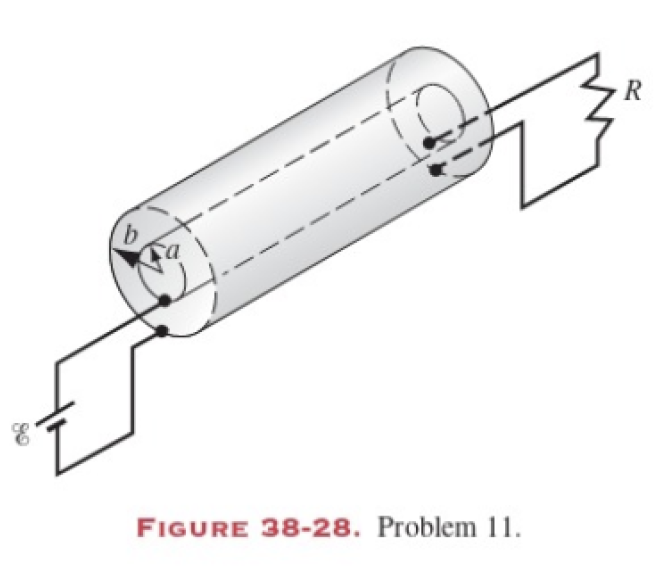
\includegraphics[scale = 0.4]{Fig_38-28}
	\end{problem}
	\clearpage



	\begin{problem}[38E14:]
		Figure 38-21 shows an $LC$ oscillator connected by a transmission line to an antenna of a magnetic dipole type.
		Compare with Fig. 38-5, which shows a similar arrangement but with an electric dipole type of antenna.
		
		\begin{center}
			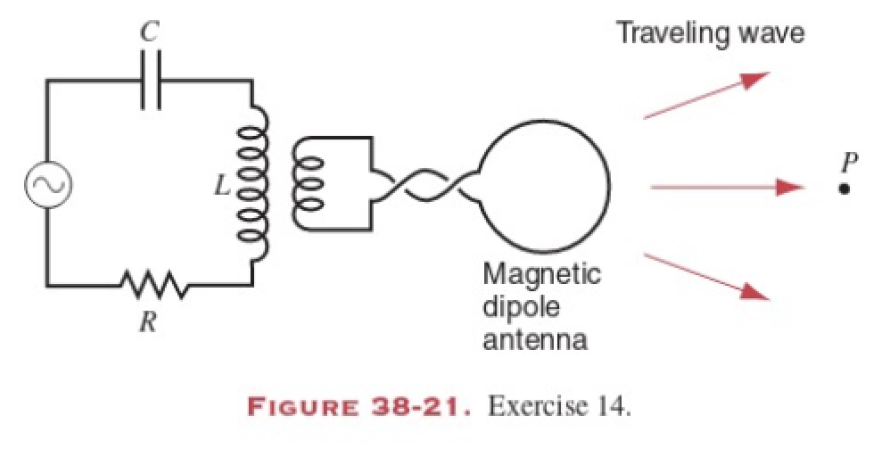
\includegraphics[scale = 0.3]{Fig_38-21} 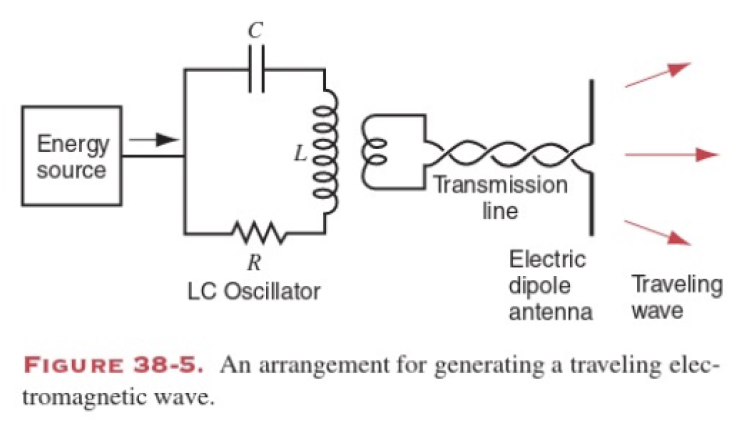
\includegraphics[scale = 0.3]{Fig_38-5}
		\end{center}

		\begin{enumerate}[(a)]
			\item What is the basis for the names of these two antenna types?
			\item Draw figures corresponding to Figs. 38-6 and 38-7 to describe the electromagnetic wave that sweeps past the observer at point $P$ in Fig. 38-21.

			\begin{center}
				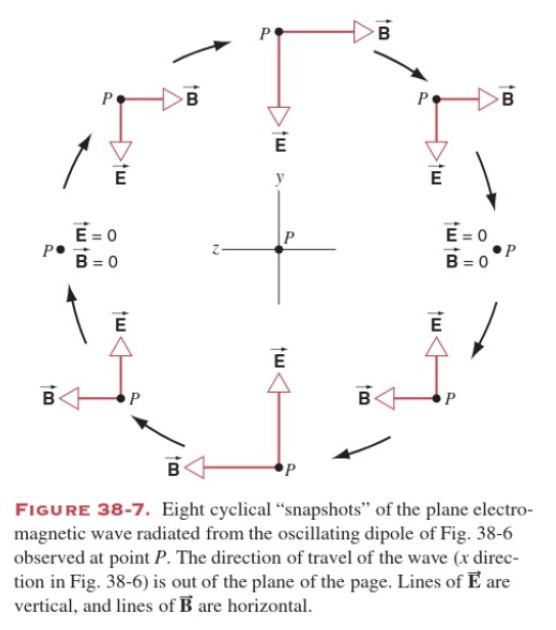
\includegraphics[scale = 0.3]{Fig_38-7} 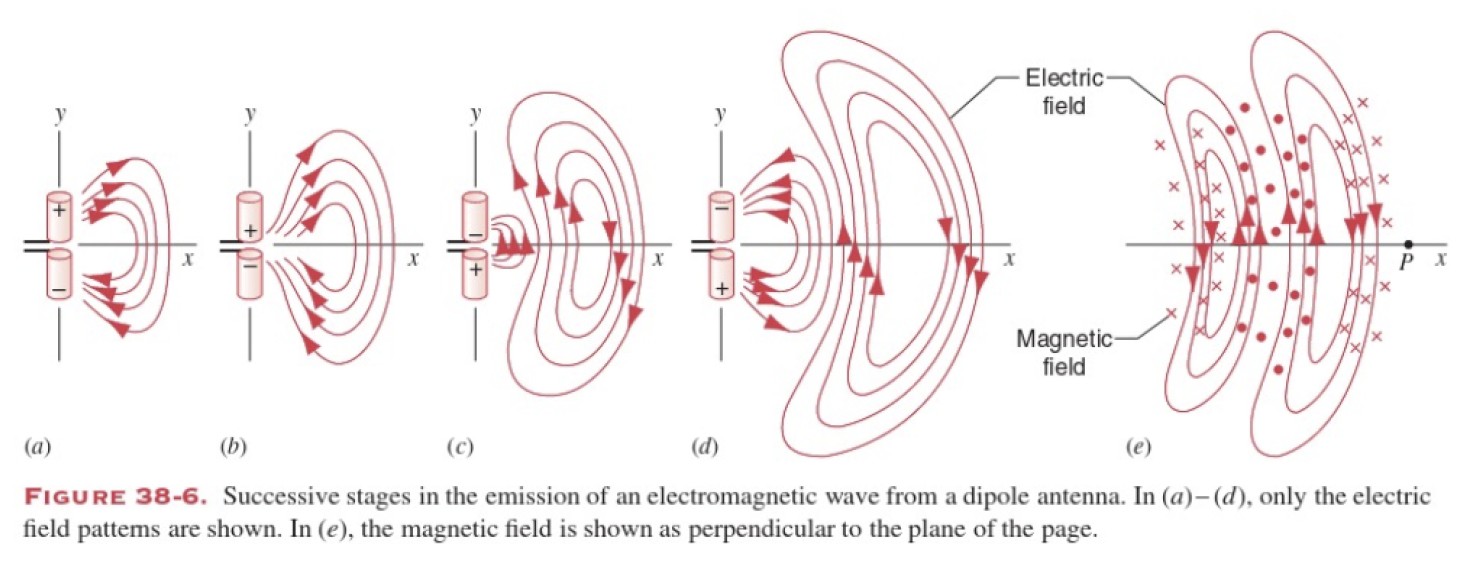
\includegraphics[scale = 0.3]{Fig_38-6}
			\end{center}
		\end{enumerate}
	\end{problem}
	\clearpage



	\begin{problem}[38E16:]
		The electric field associated with a plane electromagnetic wave is given by $E_x = 0, E_y = 0, E_z = E_0\sin{k(x - ct)}$, where $E_0 = 2.34 \times 10^{-4}$ V/m and $k = 9.72 \times 10^6$ m$^{-1}$.
		The wave is propagating in the $+x$ direction.
		\begin{enumerate}[(a)]
			\item Write expressions for the components of the magnetic field of the wave.
			\item Find the wavelength of the wave.
			\item What is the wave's frequency and what kind of radiation is it? (See Ch. 39 for a hint.)
		\end{enumerate}
	\end{problem}
	\clearpage



	\begin{problem}[38P13:]
		A plane electromagnetic wave, with wavelength 3.18 m, travels in free space in the $+x$ direction with its electric vector $\vec{\mathbf{E}}$, of amplitude 288 V/m, directed along the y axis.
		\begin{enumerate}[(a)]
			\item What is the frequency of the wave?
			\item What is the direction and amplitude of the magnetic field associated with the wave?
			\item If $E = E_m\sin{(kx - \omega t)}$, what are the values of $k$ and $\omega$?
			\item Find the intensity of the wave
			\item If the wave falls on a perfectly absorbing sheet of area 1.85 m², at what rate would momentum be delivered to the sheet and what is the radiation pressure exerted on the sheet?
		\end{enumerate}
	\end{problem}
	\clearpage



	\begin{problem}[38E42:]
		A small spaceship whose mass, with occupant, is 1500 kg is drifting in outer space, where the gravitational field is negligible.
		If the astronaut turns on a 10.0-kW laser beam, what speed would the ship attain in one day because of the reaction force associated with the momentum carried away by the beam?
	\end{problem}
	\clearpage
\end{document}